\documentclass[
11pt, % The default document font size, options: 10pt, 11pt, 12pt
codirector, % Uncomment to add a codirector to the title page
]{charter} 




% El títulos de la memoria, se usa en la carátula y se puede usar el cualquier lugar del documento con el comando \ttitle
\titulo{Gestión remota de calefactor eléctrico para el hogar} 

% Nombre del posgrado, se usa en la carátula y se puede usar el cualquier lugar del documento con el comando \degreename
%\posgrado{Carrera de Especialización en Sistemas Embebidos} 
\posgrado{Carrera de Especialización en Internet de las Cosas} 
%\posgrado{Carrera de Especialización en Intelegencia Artificial}
%\posgrado{Maestría en Sistemas Embebidos} 
%\posgrado{Maestría en Internet de las cosas}

% Tu nombre, se puede usar el cualquier lugar del documento con el comando \authorname
\autor{Ing. Leonardo Mancini} 

% El nombre del director y co-director, se puede usar el cualquier lugar del documento con el comando \supname y \cosupname y \pertesupname y \pertecosupname
\director{Mg. Ing. Diego Javier Brengi }
\pertenenciaDirector{INTI} 
% FIXME:NO IMPLEMENTADO EL CODIRECTOR ni su pertenencia
\codirector{Ing. Salvador Tropea} % para que aparezca en la portada se debe descomentar la opción codirector en el documentclass
\pertenenciaCoDirector{INTI}

% Nombre del cliente, quien va a aprobar los resultados del proyecto, se puede usar con el comando \clientename y \empclientename
\cliente{Sr. Pablo Barbero}
\empresaCliente{Intelligentgas}

% Nombre y pertenencia de los jurados, se pueden usar el cualquier lugar del documento con el comando \jurunoname, \jurdosname y \jurtresname y \perteunoname, \pertedosname y \pertetresname.
\juradoUno{Nombre y Apellido (1)}
\pertenenciaJurUno{pertenencia (1)} 
\juradoDos{Nombre y Apellido (2)}
\pertenenciaJurDos{pertenencia (2)}
\juradoTres{Nombre y Apellido (3)}
\pertenenciaJurTres{pertenencia (3)}
 
\fechaINICIO{26 de abril de 2022}		%Fecha de inicio de la cursada de GdP \fechaInicioName
\fechaFINALPlan{14 de junio de 2022} 	%Fecha de final de cursada de GdP
\fechaFINALTrabajo{16 de abril de 2023}	%Fecha de defensa pública del trabajo final


\begin{document}

\maketitle
\thispagestyle{empty}
\pagebreak


\thispagestyle{empty}
{\setlength{\parskip}{0pt}
\tableofcontents{}
}
\pagebreak


\section*{Registros de cambios}
\label{sec:registro}


\begin{table}[ht]
\label{tab:registro}
\centering
\begin{tabularx}{\linewidth}{@{}|c|X|c|@{}}
\hline
\rowcolor[HTML]{C0C0C0} 
Revisión & \multicolumn{1}{c|}{\cellcolor[HTML]{C0C0C0}Detalles de los cambios realizados} & Fecha      \\ \hline
0      & Creación del documento                                 &\fechaInicioName \\ \hline
1      & Se completa hasta el punto 5 inclusive                 & 10 de mayo de 2022\\ \hline
2      & Se completa hasta el punto 9 inclusive					 &
17 de mayo de 2022 \\ \hline
3      & Se completa hasta el punto 12 inclusive					 &
24 de mayo de 2022 \\ \hline
4      & Se completa hasta el punto 15 inclusive					 &
31 de mayo de 2022 \\ \hline
%		  Se puede agregar algo más \newline
%		  En distintas líneas \newline
%		  Así                                                    & dd/mm/aaaa \\ \hline
%3      & Se completa hasta el punto 11 inclusive                & dd/mm/aaaa \\ \hline
%4      & Se completa el plan	                                 & dd/mm/aaaa \\ \hline
\end{tabularx}
\end{table}

\pagebreak



\section*{Acta de constitución del proyecto}
\label{sec:acta}

\begin{flushright}
Buenos Aires, \fechaInicioName
\end{flushright}

\vspace{2cm}

Por medio de la presente se acuerda con el \authorname\hspace{1px} que su Trabajo Final de la \degreename\hspace{1px} se titulará ``\ttitle'', consistirá esencialmente en la implementación de un prototipo de un sistema de conexión a internet de calefactor eléctrico, y tendrá un presupuesto preliminar estimado de 600 hs de trabajo y AR\$1251500, con fecha de inicio \fechaInicioName\hspace{1px} y fecha de presentación pública \fechaFinalName.

Se adjunta a esta acta la planificación inicial. 

\vfill

% Esta parte se construye sola con la información que hayan cargado en el preámbulo del documento y no debe modificarla
\begin{table}[ht]
\centering
\begin{tabular}{ccc}
\begin{tabular}[c]{@{}c@{}}Dr. Ing. Ariel Lutenberg \\ Director posgrado FIUBA\end{tabular} & \hspace{2cm} & \begin{tabular}[c]{@{}c@{}}\clientename \\ \empclientename \end{tabular} \vspace{2.5cm} \\ 
\multicolumn{3}{c}{\begin{tabular}[c]{@{}c@{}} \supname \\ Director del Trabajo Final\end{tabular}} \vspace{2.5cm} \\
%\begin{tabular}[c]{@{}c@{}}\jurunoname \\ Jurado del Trabajo Final\end{tabular}     &  & \begin{tabular}[c]{@{}c@{}}\jurdosname\\ Jurado del Trabajo Final\end{tabular}  \vspace{2.5cm}  \\
%\multicolumn{3}{c}{\begin{tabular}[c]{@{}c@{}} \jurtresname\\ Jurado del Trabajo Final\end{tabular}} \vspace{.5cm}                                                                     
\end{tabular}
\end{table}



\pagebreak
\section{1. Descripción técnica-conceptual del proyecto a realizar}
\label{sec:descripcion}
El presente proyecto plantea desarrollar una solución IoT (Internet of 
Things) para calefactores eléctricos comercializados por la empresa Intelligentgas.
El proyecto es realizado como parte del trabajo final de la Especialización en Internet de las Cosas mediante convenio con el INTI (Instituto Nacional de Tecnología Industrial).
Actualmente la empresa comercializa soluciones IoT enfocadas en el control y monitoreo de sensores de diversos gases. La empresa tiene como objetivo ingresar al mercado de los smart home desarrollando electrodomésticos con características de IoT. El producto que se encuentra desarrollando en este momento es un calefactor eléctrico. 
En el mercado argentino no existen productos similares por lo que para la empresa es un nicho en el cual innovar.
La posibilidad de configurar en forma remota, monitorear su uso y consumo lo dotarán de una característica importante, tanto por una cuestión ambiental como comercial.
Para lograr este objetivo es que se da inicio al proyecto de brindarle conectividad a Internet mediante el desarrollo del módulo de comunicaciones. Cabe destacar que la comunicación no es el único objetivo de la solución ya que un valor agregado directamente para el cliente es la de poder tener datos que le permitirán conocer las costumbres de uso de los usuarios. 
Por lo tanto la solución planteada es una infraestructura IoT además del desarrollo del módulo Wi-Fi.

\subsection{Detalle de funcionalidad a implementar}
La solución planteada consta de:
 \begin{itemize}
 \item Módulo de comunicación Wi-Fi que permite conectar el calefactor a Internet. Mediante este módulo el calefactor podrá ser configurado y enviar datos al usuario final. La comunicación será mediante el protocolo MQTT cuyo broker se encontrará en  un servidor web. 
 \item Servidor en la nube en donde se encontrará la base de datos con información de cada calefactor y de cada usuario.
 \item Aplicación móvil mediante la cual el usuario podrá interactuar con los calefactores de su propiedad.
 \end{itemize}
 El desarrollo del sistema permitiría a cada usuario configurar y monitorear los calefactores de su propiedad. También permitirá encender/apagar los calefactores en determinado rango de tiempo y/o por distancia geográfica (si deja el hogar/está volviendo al hogar).
En la figura \ref{fig:diagBloques} se presenta el diagrama en bloques del sistema, sus principales componentes y como interactúan.
%\vspace{25px}

\begin{figure}[htpb]
\centering 
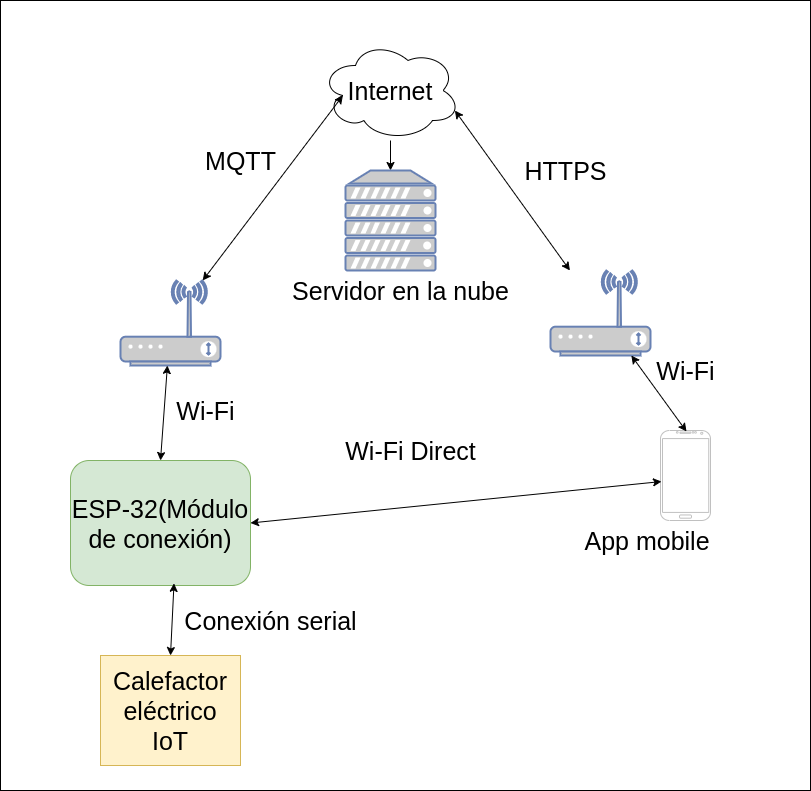
\includegraphics[width=.5\textwidth]{./Figuras/diagBloques.png}
\caption{Diagrama en bloques del sistema.}
\label{fig:diagBloques}
\end{figure}

\vspace{25px}



\section{2. Identificación y análisis de los interesados}
\label{sec:interesados}


\begin{table}[ht]
%\caption{Identificación de los interesados}
%\label{tab:interesados}
\begin{tabularx}{\linewidth}{@{}|l|X|X|l|@{}}
\hline
\rowcolor[HTML]{C0C0C0} 
Rol           & Nombre y Apellido & Organi-zación 	& Puesto 	\\ \hline
Cliente       & \clientename      &\empclientename	&     -   	\\ \hline
Responsable   & \authorname       & FIUBA        	& Alumno 	\\ \hline
Orientador    & \supname	      & \pertesupname 	& Director Trabajo final \\ \hline

Usuario final &        Usuarios de calefactores IoT           &             - 	&   -     	\\ \hline
\end{tabularx}
\end{table}

\begin{itemize}
 \item Director: muy detallista en los procesos de gestión de proyectos. Se programan las reuniones mediante meet durante el mediodía en forma semanal.
 \item Cliente: tiene conocimientos técnicos, ya cuenta con desarrollos similares. Se puede comunicar por teléfono en cualquier momento.
 También solicita guardar confidencialidad en detalles técnicos/comerciales al ser un producto comercial.
\end{itemize}



\section{3. Propósito del proyecto}
\label{sec:proposito}

\begin{consigna}{black}
El propósito de este proyecto es brindar funcionalidad IoT a los calefactores comercializados por la empresa del cliente. El objetivo se logrará con el desarrollo de un módulo de comunicaciones Wi-Fi que permitirá enviar y recibir eventos entre un servidor en la nube y el calefactor. De esta forma se podrá monitorear e interactuar en forma remota y lograr un uso más eficiente del calefactor.
\end{consigna}

\section{4. Alcance del proyecto}
\label{sec:alcance}

\begin{consigna}{black}
El desarrollo del presente proyecto incluye:
\begin{itemize}

	\item Desarrollo de firmware para el módulo de conexión Wi-Fi.
	\item Desarrollo de una aplicación móvil hibrida para el usuario final que permitirá monitorear/configurar el calefactor.
	\item Desarrollo del servidor en la nube.
	\item Construcción del prototipo de hardware.
\end{itemize}	
El desarrollo no incluirá:
\begin{itemize}
	\item Construcción del producto final.
	\item Gestión de usuarios con Third Party.
	\item Distribución comercial de las aplicaciones.
\end{itemize}
\end{consigna}


\section{5. Supuestos del proyecto}
\label{sec:supuestos}

\begin{consigna}{black}
Para el desarrollo del presente proyecto se supone que:

\begin{itemize}
	\item El cliente proveerá el hardware controlador del calefactor.
	\item El cliente proveerá el hardware de conexión Wi-Fi (Módulo ESP-32).
	\item El cliente proveerá acceso a los servidores de Google Cloud Plattform.
	\item Durante el cursado de la especialidad se obtendrán los conocimientos necesarios para lograr el objetivo.
	\item Se dispondrá del acceso a los repositorios de Android/IoS para la publicación.
\end{itemize}


\end{consigna}

\section{6. Requerimientos}
\label{sec:requerimientos}

\begin{consigna}{black}

\begin{enumerate}
	\item Requerimientos funcionales:
		\begin{enumerate}
			\item El usuario podrá dar de alta, baja y modificar información (dirección, nombre y descripción) de los  calefactores en el sistema.
			
			\item El usuario podrá establecer el valor de la temperatura del calefactor en grados centígrados.
			\item El usuario podrá configurar hora y fecha de encendido y apagado de cada calefactor.
			\item El usuario podrá configurar una distancia de apagado/encendido automático en un rango de 1-50 km.
			\item El usuario podrá establecer el valor de kWh (Kilo-watt hora).
			\item El usuario podrá consultar el consumo de energía en kWh en el mes en curso.
			\item Se deberá registrar las coordenadas geográficas de cada calefactor en el sistema.
		\end{enumerate}
	\item Requerimientos del  módulo embebido:
		\begin{enumerate}
			\item Se podrá configurar la red Wi-Fi.
			\item Se podrá configurar el reloj interno.
			\item La comunicación con la electrónica del calefactor deberá ser serial.
			\item Deberá informar los datos de temperatura al servidor cada 10 segundos.
			\item En caso de mal funcionamiento, no detectar temperatura, informará el error mediante MQTT al servidor.
		\end{enumerate}
	\item Requerimientos de comunicaciones:
		\begin{enumerate}
			\item El calefactor permitirá ser configurado mediante Wi-Fi Direct.
			\item El calefactor podrá ser accedido mediante Internet para ser configurado y mostrar la temperatura actual.
			\item El protocolo de comunicación entre servidor y calefactor deberá ser bi-direccional mediante MQTT.
			\item Las rutas MQTT para identificar cada calefactor deberán seguir una jerarquia: /usuario/{usuario}/ubicacion/{ubicacion}/calefactor/{calefactor}.
			\item La comunicación entre el dispositivo móvil y el servidor deberá ser mediante APIs REST.
			\item El servidor, si está configurado el aviso por cercanía, enviará el evento al calefactor.
		\end{enumerate}
	
	\item Requerimientos de la aplicación móvil:
		\begin{enumerate}
			\item La aplicación móvil deberá mostrar un listado de calefactores del usuario conectado.
			\item La aplicación móvil deberá mostrar la temperatura actual del ambiente y los valores de configuración del calefactor.
			\item La aplicación móvil permitirá ingresar el costo del kWh en el sistema para calcular costos de consumo.
			\item La aplicación móvil mostrará el consumo en kW
			 y el costo en pesos acumulados en el mes actual.
			\item La aplicación móvil permitirá recibir y mostrar notificaciones cuando ocurre un evento con alguno de los calefactores.
			\item Deberá tener una pantalla de ingreso a la aplicación.
			\item La aplicación móvil deberá capturar las coordenadas de GPS con una frecuencia de 10 minutos.
			\item La aplicación móvil deberá calcular si se encuentra geográficamente en el rango de la ubicación del calefactor y en caso afirmativo enviar evento al servidor.
			
		\end{enumerate}
	\item Requerimientos no funcionales:
		\begin{enumerate}
			\item El módulo de comunicaciones deberá permitir la configuración de red Wi-Fi mediante WPS.
			\item El servidor, con el broker y su base de datos deberán estar alojados en un entorno cloud.
			\item Los datos enviados por MQTT deberán estar estar cifrados con TLS.
			\item La comunicación con la API Rest deberá ser mediante HTTPS.
		
			
		\end{enumerate}
	
\end{enumerate}



\end{consigna}
\pagebreak
\section{7. Historias de usuarios (\textit{Product backlog})}
\label{sec:backlog}

\begin{consigna}{black}
La ponderación de las historias de usuario se realizará a través de story
points. Para determinar el puntaje para cada historia se evaluará cada una de ellas de acuerdo a tres aspectos: cantidad de trabajo a realizar, complejidad e incertidumbre. Por cada aspecto se utilizarán las siguientes escalas:
	\begin{itemize}
	\item Cantidad de trabajo:
		\begin{itemize}
		\item Alta: 8
		\item Media: 5
		\item Baja 1
		\end{itemize}
	\item Complejidad:
		\begin{itemize}
		\item Alta: 8
		\item Media: 5
		\item Baja: 1
		\end{itemize}
	\item Incertidumbre:
		\begin{itemize}
		\item Alta: 5
		\item Media: 3
		\item Baja: 0
		\end{itemize}
	\end{itemize}

Se utilizará la escala de Fibonacci para determinar el puntaje final: {0,1,1,2,3,5,8,13,21}. 
Utilizando estas escalas y evaluando los tres aspectos, se procede a sumar el puntaje final, redondeando al próximo valor de Fibonacci más cercano. Si el puntaje supera los 21 puntos, la historia deberá dividirse en historias más pequeñas.
\begin{enumerate}
	\item Como usuario del calefactor quiero  configurar la temperatura del mismo para que el calefactor pueda calefaccionar el ambiente donde se ubica.
		\begin{itemize}
		\item Cantidad de trabajo: media
		\item Complejidad: media
		\item Incertidumbre: baja
		\item Puntos: \textit{13}
		\end{itemize}
		
	\item Como usuario del calefactor quiero configurar hora de encendido y apagado para poder programar la calefacción del hogar.
		\begin{itemize}
		\item Cantidad de trabajo: media
		\item Complejidad: media
		\item Incertidumbre: media
		\item Puntos: \textit{13}
		\end{itemize}
	\item Como usuario del calefactor quiero recibir notificaciones de mal funcionamiento para poder saber que el calefactor ha dejado de funcionar en el momento que suceda.
		\begin{itemize}
		\item Cantidad de trabajo: alta
		\item Complejidad: media
		\item Incertidumbre: media
		\item Puntos: \textit{21}
		\end{itemize}

	\item Como usuario del calefactor quiero configurar el valor, en pesos, del kWh para que se puedan realizar los gastos en un periodo de tiempo.
		\begin{itemize}
		\item Cantidad de trabajo: baja
		\item Complejidad: baja
		\item Incertidumbre: baja
		\item Puntos: \textit{2}
		\end{itemize}
	\item Como usuario del calefactor quiero obtener el consumo de electricidad mensual para poder obtener los gastos en un periodo de tiempo.
		\begin{itemize}
		\item Cantidad de trabajo: media
		\item Complejidad: baja
		\item Incertidumbre: baja
		\item Puntos: \textit{8}
		\end{itemize}
	\item Como usuario del calefactor quiero activar el apagado automático por distancia geográfica para poder automatizar cuando salgo del hogar.
		\begin{itemize}
		\item Cantidad de trabajo: baja
		\item Complejidad: baja
		\item Incertidumbre: media
		\item Puntos: \textit{5}
		\end{itemize}
\end{enumerate}




\end{consigna}

\pagebreak
\section{8. Entregables principales del proyecto}
\label{sec:entregables}

\begin{consigna}{black}
En esta sección se listan los entregables del proyecto. Cada uno de estos items constituye un hito en el proyecto.
\begin{itemize}
	\item Broker MQTT instalado y configurado.
	\item Repositorios de código fuente del módulo de comunicaciones, backend y aplicación híbrida.
	\item Base de datos del servidor.
	\item API RESTs para el backend.
	\item Prototipo funcional de la aplicación para el usuario final.
	\item Memoria final del proyecto.
	\item Informe de avance.
	\item Scripts para generación de la aplicación.
	\item Diagrama de la arquitectura de la solución.
\end{itemize}

\end{consigna}
\pagebreak
\section{9. Desglose del trabajo en tareas}
\label{sec:wbs}
\begin{consigna}{black}
\begin{enumerate}
\item Planificación del proyecto.
	\begin{enumerate}
	\item Escritura del plan de proyecto (40 hs).
	\end{enumerate}
\item Investigación preliminar.
	\begin{enumerate}
	\item Investigación de la placa controladora: como conectarla en serie al módulo Wi-Fi y el formato de la trama de datos enviados (30 hs).
	\item Investigación sobre la configuración WPS del módulo Wi-Fi (20 hs).
	\item Investigación sobre la configuración del protocolo MQTT en modulo Wi-Fi (10 hs). 
	\end{enumerate}
\item Desarrollo de firmware (embebido en módulo Wi-Fi).
	\begin{enumerate}

	\item Desarrollar módulos de conectividad Wi-Fi y Wi-Fi Direct (20 hs).
	\item Desarrollar el módulo de comunicación serial con calefactor eléctrico (20 hs).
	\item Desarrollo de módulo MQTT (35 hs).
	\item Desarrollo de la configuración del clock interno de módulo Wi-Fi (20 hs).
	\item Prueba de configuración y conexión del módulo WI-Fi (20 hs).
	
	\end{enumerate}
\item Construcción de prototipo.
	\begin{enumerate}
	\item Realizar conectividad por hardware entre el módulo Wi-Fi y la placa controladora del calefactor(4 hs).
	\item Verificar conectividad y lectura de datos de la controladora ( 6 hs).
	
	\end{enumerate}
\item Desarrollo de backend.
	\begin{enumerate}
	\item Implementación del modelo de base de datos (35 hs).
	\item Instalación y configuración del broker MQTT (15 hs).
	
	\item Pruebas del broker MQTT, verificar conexión con prototipo. (20 hs)
	\item Desarrollo de la API REST (40 hs).
	\item Desarrollo del diagrama de arquitectura de la solución ( 20 hs).
	\item Desarrollo del módulo de mensajería para envío de notificaciones ( 30 hs).
	
	\item Verificar funcionamiento de la API REST (20 hs).
	
	\end{enumerate}
	\item Desarrollo de aplicación móvil.
	\begin{enumerate}
	
	\item Crear script para el despliegue (5 hs).
	\item Desarrollar la pantalla de ingreso (5 hs).
	\item Desarrollar la funcionalidad de gestión de calefactores: alta, baja y modificación (30 hs).
	\item Desarrollar la pantalla de configuración de conectividad del calefactor (Mediante Wi-Fi direct) (15 hs).
	\item Desarrollar la funcionalidad de configuración de temperatura ambiente y estado  del calefactor (10 hs).
	\item Desarrollar la funcionalidad de programación de encendido/apagado del calefactor (20 hs).
	\item Desarrollo de la pantalla de control de encendido/apagado por distancia geográfica (2 hs).
	\item Desarrollo de módulo de recepción de notificaciones (15 hs).
	\item Implementar la comunicación HTTPS con el backend (15 hs).
	\item Verificar el funcionamiento de la aplicación con pruebas de integración end-to-end (30 hs).
	
	\end{enumerate}
	
	\item Documentación del proyecto.
	\begin{enumerate}
	\item Redacción del informe de avances (10 hs)
	\item Escritura de memoria final (40 hs).
	\item Preparación de la presentación del proyecto (20 hs).
	\end{enumerate}
	
	
\end{enumerate}

Cantidad total de horas: (641 hs).



\end{consigna}
\pagebreak
\section{10. Diagrama de Activity On Node}
\label{sec:AoN}

En la figura 2 se muestra el diagrama de las actividades del proyecto y su camino crítico. La unidad de tiempo utilizada son horas.
\begin{figure}[htpb]
\centering 
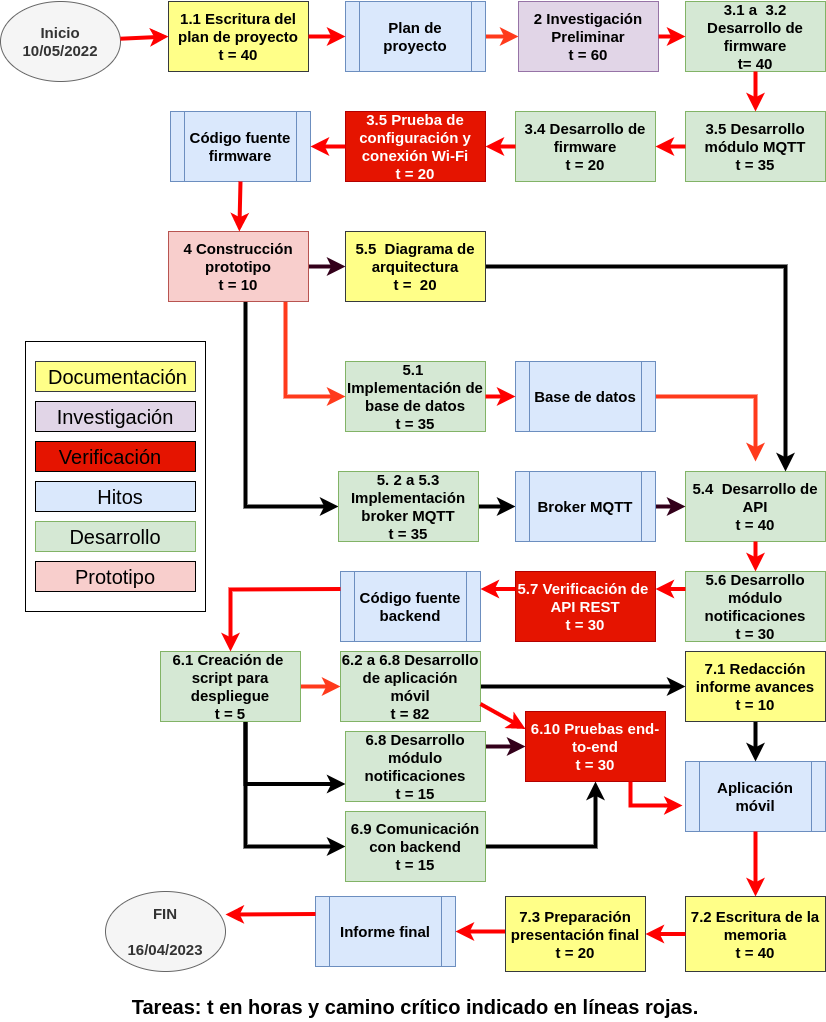
\includegraphics[width=.8\textwidth]{./Figuras/AoN.png}
\caption{Diagrama en \textit{Activity on Node}}
\label{fig:AoN}
\end{figure}




\pagebreak
\section{11. Diagrama de Gantt}
\label{sec:gantt}

\begin{consigna}{black}
En esta sección se detalla el diagrama de Gantt del proyecto. 
A continuación se muestra el listado de las tareas e hitos del proyecto.

\begin{figure}[htpb]

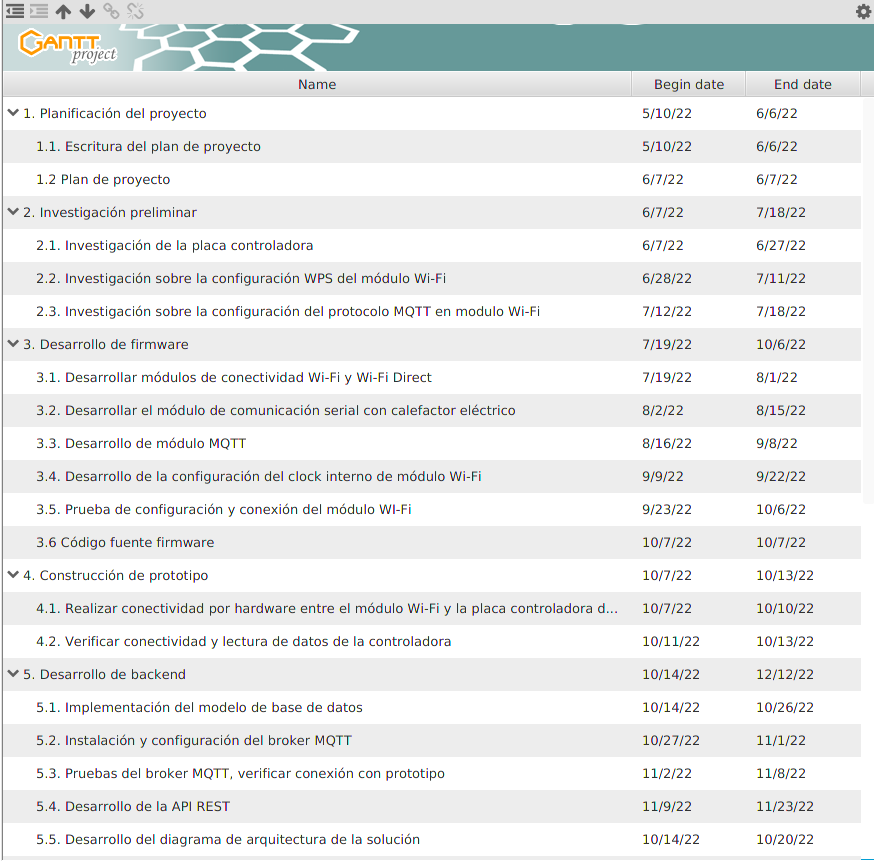
\includegraphics[width=1.0\textwidth]{./Figuras/planificacion-1.png}
\caption{Listado de tareas.}
\label{fig:AoN}
\end{figure}
\begin{figure}[htpb]

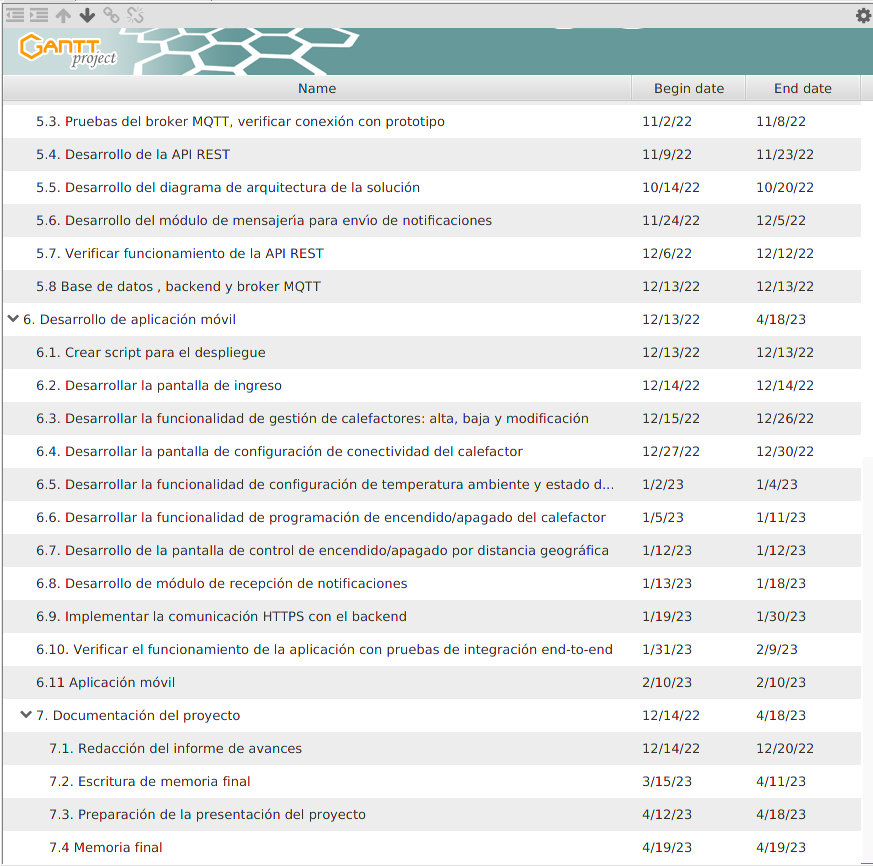
\includegraphics[width=1.0\textwidth]{./Figuras/planificacion-2.png}
\caption{Listado de tareas.}
\label{fig:AoN}
\end{figure}

\begin{landscape}
\begin{figure}[htpb]

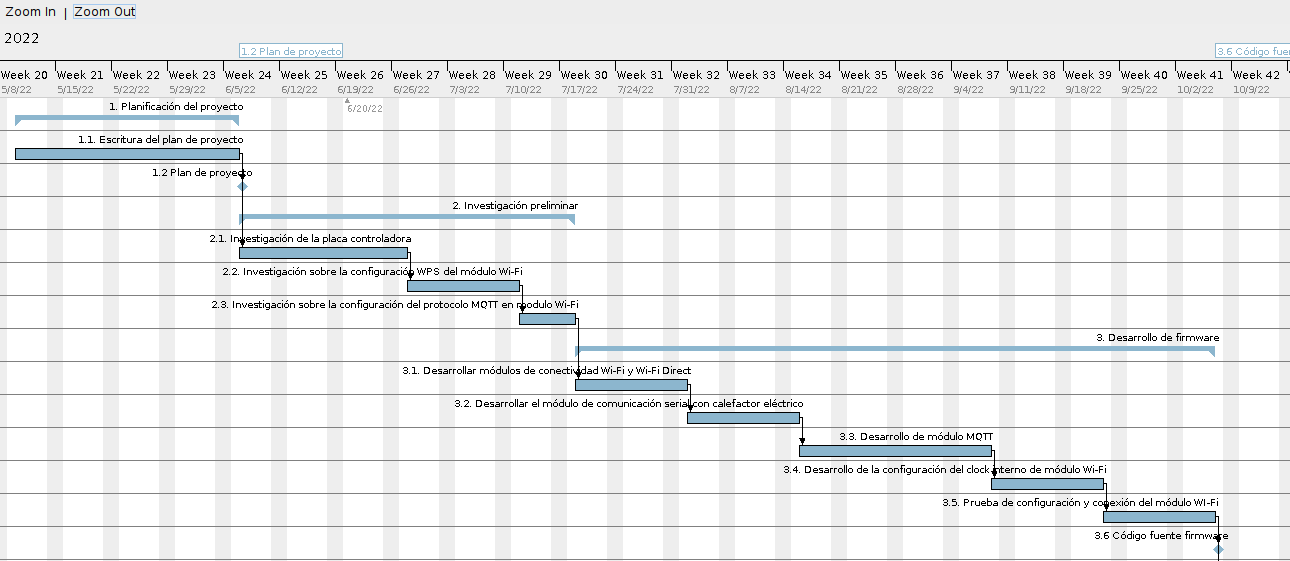
\includegraphics[height=.65\textheight]{./Figuras/gantt-1.png}
\caption{Diagrama de Gantt. }
\label{fig:diagGantt}
\end{figure}

\end{landscape}
\begin{landscape}
\begin{figure}[htpb]
\centering 
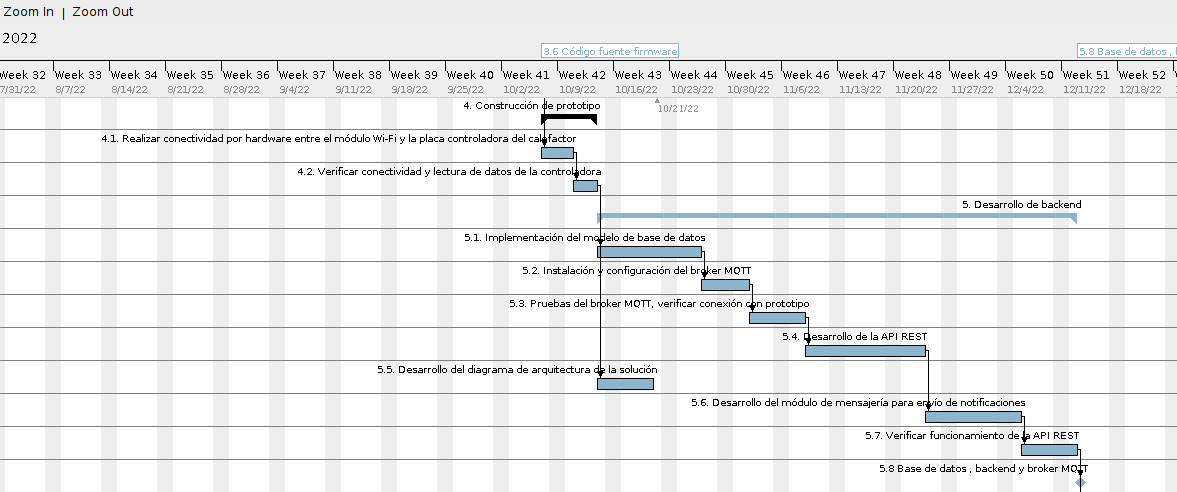
\includegraphics[height=.65\textheight]{./Figuras/gantt-2.png}
\caption{Diagrama de Gantt. }
\label{fig:diagGantt}
\end{figure}

\end{landscape}

\begin{landscape}
\begin{figure}[htpb]
\centering 
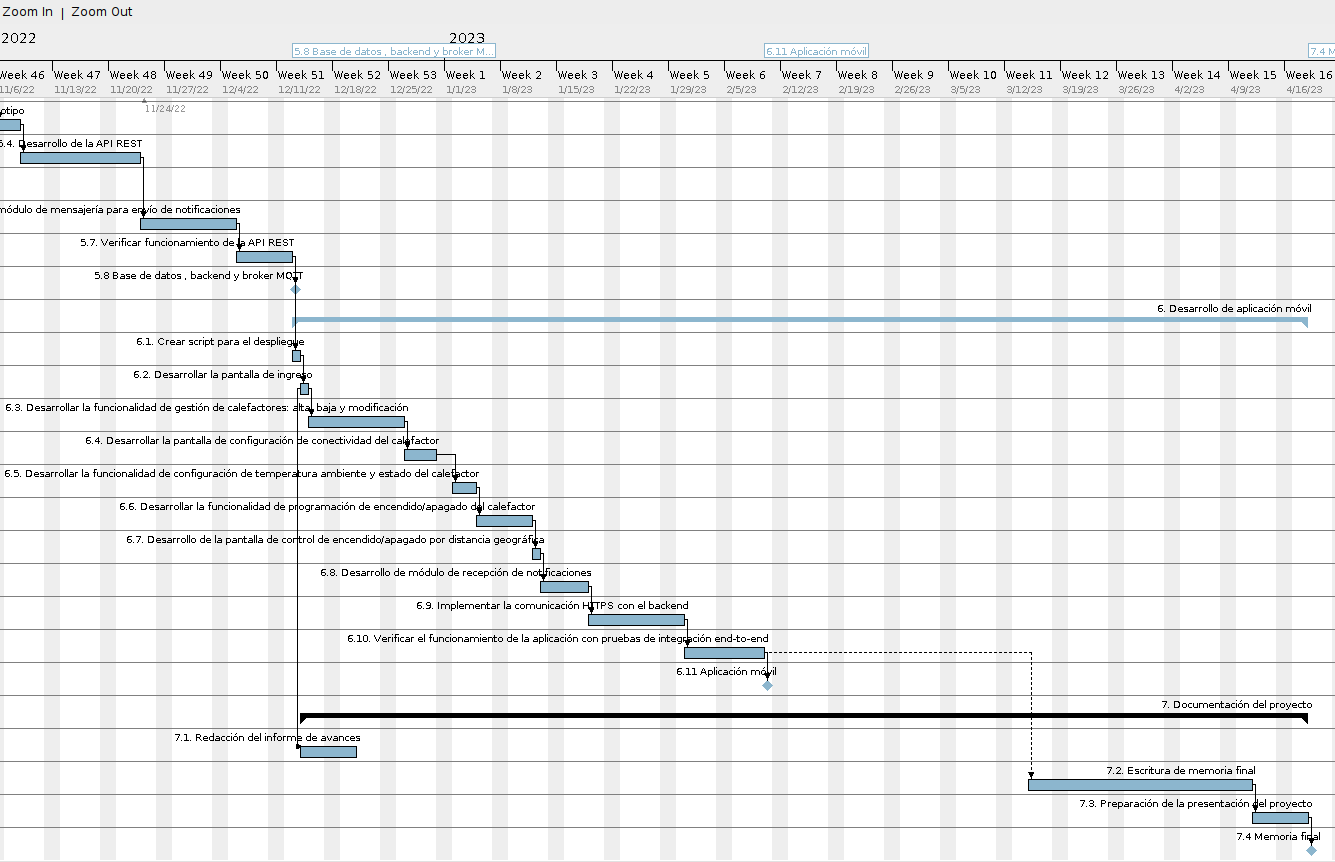
\includegraphics[height=1.0\textheight]{./Figuras/gantt-3.png}
\caption{Diagrama de Gantt.}
\label{fig:diagGantt}
\end{figure}

\end{landscape}


\end{consigna}

\pagebreak
\section{12. Presupuesto detallado del proyecto}
\label{sec:presupuesto}

A continuación se detallan los costos asociados el proyecto expresados en pesos argentinos (AR\$).

\begin{table}[htpb]
\centering
\begin{tabularx}{\linewidth}{@{}|X|c|r|r|@{}}
\hline
\rowcolor[HTML]{C0C0C0} 
\multicolumn{4}{|c|}{\cellcolor[HTML]{C0C0C0}COSTOS DIRECTOS} \\ \hline
\rowcolor[HTML]{C0C0C0} 
Descripción &
  \multicolumn{1}{c|}{\cellcolor[HTML]{C0C0C0}Cantidad} &
  \multicolumn{1}{c|}{\cellcolor[HTML]{C0C0C0}Valor unitario} &
  \multicolumn{1}{c|}{\cellcolor[HTML]{C0C0C0}Valor total} \\ \hline

  Horas de trabajo &
  657 &
  \$1500 &
  \$985500 \\ \hline
 
  Módulo esp-32 &
  1 &
  \$3000 &
\$3000\\ \hline
 Hardware prototipo controlador del calefactor &
  1 &
  \$20000 &
\$20000 \\ \hline

\multicolumn{3}{|c|}{SUBTOTAL} &
  \$1008500 \\ \hline
\rowcolor[HTML]{C0C0C0} 
\multicolumn{4}{|c|}{\cellcolor[HTML]{C0C0C0}COSTOS INDIRECTOS} \\ \hline
\rowcolor[HTML]{C0C0C0} 
Descripción &
  \multicolumn{1}{c|}{\cellcolor[HTML]{C0C0C0}Cantidad} &
  \multicolumn{1}{c|}{\cellcolor[HTML]{C0C0C0}Valor unitario} &
  \multicolumn{1}{c|}{\cellcolor[HTML]{C0C0C0}Valor total} \\ \hline
\multicolumn{1}{|l|}{Conexión mensual a Internet} &10
   & \$4000
   &\$40000
   \\ \hline
   \multicolumn{1}{|l|}{Matricula posgrado } &1
   & \$40000
   &\$40000
   \\ \hline
     \multicolumn{1}{|l|}{Cuota posgrado } &10
   & \$16300
   &\$163000
    \\ \hline
     \multicolumn{1}{|l|}{30\% sobre costos directos } &1
   & \$302550
   &\$302550
   \\ \hline

\multicolumn{3}{|c|}{SUBTOTAL} &
  \$545550 \\ \hline
\rowcolor[HTML]{C0C0C0}
\multicolumn{3}{|c|}{TOTAL} &\$1554050
   \\ \hline
\end{tabularx}
\end{table}

\pagebreak
\section{13. Gestión de riesgos}
\label{sec:riesgos}

\begin{consigna}{black}

Riesgo 1: demora en obtener la placa controladora del calefactor.
\begin{itemize}
	\item Severidad (6): la demora en obtener la placa controladora retrasaría el inicio del proyecto ya que es necesaria para las primeras tareas planificadas.
	\item Probabilidad de ocurrencia (2): probabilidad baja ya que se ha coordinado con el cliente el envío de la placa controladora para que esté disponible en las primeras semanas de junio. 
\end{itemize}   

Riesgo 2: aumento de costos de módulo Wi-Fi.
\begin{itemize}
	\item Severidad (8): el módulo Wi-Fi es un componente importante en el proyecto, no poder adquirirlo provocaría tener que re definir la tecnología a utilizar. 
	\item Ocurrencia (6): los precios de placas controladoras y componentes de hardware han tenido aumentos importantes en los últimos meses.
\end{itemize}

Riesgo 3: demora en implementar servicios cloud con la tecnología seleccionada.
\begin{itemize}
	\item Severidad (6): la demora en implementar servicios REST y broker MQTT provocaría que el proyecto se extienda en el tiempo estipulado.
	\item Ocurrencia (5): al ser una tecnología nueva para el equipo de desarrollo es probable que se produzcan bloqueos por falta de conocimiento.
\end{itemize}

Riesgo 4: los requerimientos tienen una mayor complejidad que la esperada.
\begin{itemize}
	\item Severidad (7): el proyecto demandaría mas tiempo del estimado.
	\item Ocurrencia (3): falta de conocimientos del tema seleccionado.
\end{itemize}

Riesgo 5: el cliente decide no continuar el proyecto.
\begin{itemize}
	\item Severidad (9):  la decisión del cliente de no continuar el proyecto por decisión unilateral provocaría que tenga que redefinirse el plan.
	\item Ocurrencia (2): el cliente está muy comprometido con el proyecto y los tiempos planificados son acordes a sus expectativas.
\end{itemize}

Tabla de gestión de riesgos:      (El RPN se calcula como RPN=SxO)

\begin{table}[htpb]
\centering
\begin{tabularx}{\linewidth}{@{}|X|c|c|c|c|c|c|@{}}
\hline
\rowcolor[HTML]{C0C0C0} 
Riesgo & S & O & RPN & S* & O* & RPN* \\ \hline
 1. Demora en obtener placa      & 6  & 2  &  12   &    &    &      \\ \hline
 2. Aumento de costo del módulo Wi-Fi      &  8 &  6 &  48   &  7  &  3  &     21 \\ \hline
 3. Demora en implementar servicios cloud      & 6  &  5 &  30   &  4  &   3 &    12  \\ \hline
  4. Mayor complejidad en los requerimientos     & 7  &  3 &  21   &    &    &      \\ \hline
 5. Cliente decide no continuar      & 9  &  2 &  18   &    &    &      \\ \hline
\end{tabularx}%
\end{table}

Criterio adoptado: 
Se tomarán medidas de mitigación en los riesgos cuyos números de RPN sean mayores a 30.

Nota: los valores marcados con (*) en la tabla corresponden luego de haber aplicado la mitigación.

Plan de mitigación de los riesgos que originalmente excedían el RPN máximo establecido:
 
Riesgo 2: se cuenta con módulos Wi-Fi propios a modo de respaldo.
  
  \begin{itemize}
  \item Severidad (7): en caso de aumentar el precio se pueden utilizar los módulos ya adquiridos para otros proyectos. Se debe tener cuidado de no dañarlos para evitar tener que comprar nuevos módulos.
  \item Probabilidad de ocurrencia (3): es poco probable que se rompan los módulos asignados.
  \end{itemize}
 
Riesgo 3: adquirir conocimientos de la tecnología a utilizar mediante los temas vistos en las materias de la especialidad. Realizar consultas de dudas con expertos en la materia.
	\begin{itemize}
	\item Severidad (4): se reducirá la demora en tener listos los servicios cloud al contar con los conocimientos tecnicos y la posibilidad de realizar consultas técnicas.
	\item Probabilidad de ocurrencia (3): los bloqueos se van a reducir ya que en la etapa de construcción de servicios cloud ya se contará con los conocimientos necesarios.
	\end{itemize} 


\end{consigna}

\pagebreak
\section{14. Gestión de la calidad}
\label{sec:calidad}

\begin{consigna}{black}

\begin{itemize} 
\item Requerimiento \#1.1: el usuario podrá dar de alta, baja y modificar información (dirección, nombre
y descripción) de los calefactores en el sistema.

\begin{itemize}
	\item Verificación: debe existir una pantalla en la aplicación que permita agregar, eliminar y modificar datos de calefactores. 
	\item Validación: realizar mediante la aplicación las operaciones y deberán poder verse en la pantalla.
\end{itemize}

\item Requerimiento \#1.2: el calefactor deberá medir la temperatura ambiente en grados centígrados y con una
precisión de +-0.5 ° C.

\begin{itemize}
	\item Verificación: revisar las especificaciones técnicas del sensor de medición de temperatura. 
	\item Validación: no aplica.
\end{itemize}


\item Requerimiento \#1.3: el usuario podrá establecer el valor de la temperatura del calefactor en grados centígrados.

\begin{itemize}
	\item Verificación: la aplicación debe tener incluida pantalla para establecer temperatura.
	\item Validación: utilizando la aplicación configurar la temperatura del calefactor.
\end{itemize}

\item Requerimiento \#1.4: el usuario podrá configurar hora y fecha de encendido y apagado de cada calefactor.

\begin{itemize}
	\item Verificación: la aplicación debe tener incluida pantalla para la programación de encendido y apagado de calefactores.
	\item Validación: utilizando la aplicación programar el encendido y apagado de un calefactor.
\end{itemize}

\item Requerimiento \#1.5: el usuario podrá configurar una distancia de apagado/encendido automático en un rango de 1-50 km.

\begin{itemize}
	\item Verificación: la aplicación deber tener incluida pantalla para configurar distancia/apagado por distancia. Los valores permitidos deben ser en el rango de 1 a 5 kms.
	\item Validación: utilizando la aplicación configurar una distancia de encendido/apagado.
\end{itemize}

\item Requerimiento \#1.6: el usuario podrá establecer el valor de kWh (Kilo-watt hora).

\begin{itemize}
	\item Verificación: la aplicación debe tener incluida pantalla para establecer el valor de kWh (Kilo-watt hora).
	\item Validación: utilizando la aplicación establecer el valor de kWh (Kilo-watt hora) y poder ver la configuración en la pantalla.
\end{itemize}

\item Requerimiento \#1.7: el usuario podrá consultar el consumo de energía en kWh en el mes en curso.

\begin{itemize}
	\item Verificación: el servidor debe almacenar el tiempo de encendido de cada calefactor del usuario.
	\item Validación: utilizando la aplicación ver el consumo por pantalla.
\end{itemize}

\item Requerimiento \#1.8: se deberá registrar las coordenadas geográficas de cada calefactor en el sistema.

\begin{itemize}
	\item Verificación: la aplicación debe tener campos para ingresar las coordenadas geográficas de ubicación de un calefactor y deben almacenarse en la base de datos.
	\item Validación: utilizando la aplicación ingresar coordenadas de latitud y longitud y poder verlas por pantalla.
\end{itemize}

\item Requerimiento \#2.1: se podrá configurar la red Wi-Fi.

\begin{itemize}
	\item Verificación: el firmware del módulo Wi-Fi debe permitir configurar SSID y password de red Wi-Fi. Configurar mediante comandos y verificar que se conecte a Internet. 
	\item Validación: utilizando la aplicación configurar el Wi-Fi del calefactor y comprobar que se conecte a Internet.
\end{itemize}

\item Requerimiento \#2.2: se podrá configurar el reloj interno.

\begin{itemize}
	\item Verificación: el firmware del módulo Wi-Fi debe tener lógica de sincronismo NTP. Monitorear por puerto serial la fecha sincronizada.  
	\item Validación: no aplica.
\end{itemize}

\item Requerimiento \#2.3: la comunicación con la electrónica del calefactor deberá ser serial.

\begin{itemize}
	\item Verificación: revisar esquemático de conexión entre modulo Wi-Fi y placa controladora. Observar por puerto serie los datos entregados por la placa controladora y compararlos con la trama esperada.
	\item Validación: Enviarle al cliente la trama recibida de la placa controladora para que la valide.
\end{itemize}

\item Requerimiento \#2.4: deberá informar los datos de temperatura al servidor cada 10 segundos.

\begin{itemize}
	\item Verificación: el firmware del módulo Wi-Fi debe tener una tarea que se ejecute cada 10 segundos y envíe el valor de temperatura al servidor.
	\item Validación: no aplica.
\end{itemize}

\item Requerimiento \#2.5: en caso de mal funcionamiento, no detectar temperatura, informará el error mediante MQTT al servidor.

\begin{itemize}
	\item Verificación: el firmware del módulo Wi-Fi debe tener lógica de evento de no detección de temperatura. Para simular evento se desconectará la conexión entre placa controladora y módulo Wi-Fi. Se verificará finalmente que en el servidor MQTT exista el evento.
	\item Validación: no aplica.
\end{itemize}

\item Requerimiento \#3.1: el calefactor permitirá ser configurado mediante Wi-Fi Direct.

\begin{itemize}
	\item Verificación: el módulo Wi-Fi debe permitir conexión Wi-Fi Direct. La aplicación deberá tener opción de conectarse mediante Wi-Fi Direct.
	\item Validación: desde la aplicación conectarse mediante Wi-Fi direct a un calefactor.
\end{itemize}

\item Requerimiento \#3.2: el calefactor podrá ser accedido mediante Internet para ser configurado y mostrar la temperatura actual.

\begin{itemize}
	\item Verificación: el módulo Wi-Fi pueda ser accedido desde Internet. 
	\item Validación: desde la aplicación conectarse mediante Internet a un calefactor.
\end{itemize}

\item Requerimiento \#3.3: el protocolo de comunicación entre servidor y calefactor deberá ser bi-direccional mediante MQTT.

\begin{itemize}
	\item Verificación: el módulo Wi-Fi debe tener lógica de conexión mediante MQTT, lógica de publicación y suscripción. 
	\item Validación: no aplica.
\end{itemize}

\item Requerimiento \#3.4: las rutas MQTT para identificar cada calefactor deberán seguir una jerarquia:/usuario/usuario/ubicacion/ubicacion/calefactor/calefactor.

\begin{itemize}
	\item Verificación: el módulo Wi-Fi debe enviar datos mediante MQTT a la ruta  /usuario/usuario/ubicacion/ubicacion/calefactor/calefactor. Verificar en broker MQTT la existencia de la ruta una vez que el calefactor publique datos.
	\item Validación: no aplica.
\end{itemize}

\item Requerimiento \#3.5: la comunicación entre el dispositivo móvil y el servidor deberá ser mediante APIs REST.

\begin{itemize}
	\item Verificación: el servidor cloud deberá incluir endpoints para la comunicación con la aplicación. Ejecutar requests con un cliente REST y verificar que los response sean los esperados por la aplicación.
	\item Validación: no aplica.
\end{itemize}

\item Requerimiento \#3.6: el servidor, si está configurado el aviso por cercanía, deberá enviar el evento al calefactor.

\begin{itemize}
	\item Verificación: configurar un calefactor para que pueda ser encendido mediante evento de cercanía. Enviar mediante endpoint REST evento de encendido por cercanía. El servidor debe enviar mediante MQTT evento de encendido al calefactor.
	\item Validación: no aplica.
\end{itemize}

\item Requerimiento \#4.1: la aplicación móvil deberá mostrar un listado de calefactores del usuario conectado.

\begin{itemize}
	\item Verificación: la aplicación deberá tener una pantalla donde se listen los calefactores asociados al usuario.
	\item Validación: ingresar a la aplicación y dar de alta uno o varios calefactores. Luego validar que esos calefactores aparezcan en la pantalla de listado de calefactores.
\end{itemize}

\item Requerimiento \#4.2: la aplicación móvil mostrará la temperatura actual del ambiente y los valores de configuración del calefactor.

\begin{itemize}
	\item Verificación: la aplicación deberá tener una pantalla donde se pueda consultar la temperatura ambiente y valores de configuración para un calefactor seleccionado. Verificar que los datos mostrados sean los mismos a los datos almacenados en la base de datos.
	\item Validación: ingresar a la aplicación y seleccionar un calefactor.  Ver los datos del calefactor en la pantalla.
\end{itemize}

\item Requerimiento \#4.3: la aplicación móvil deberá permitir ingresar el costo del kWh en el sistema para calcular costos de consumo.

\begin{itemize}
	\item Verificación: la aplicación deberá tener una pantalla donde se pueda ingresar el costo en pesos del kWh.
	\item Validación: ingresar a la pantalla de configuración de costo de kWh y establecer un valor. Ver en la pantalla mensaje de configuración exitosa.
\end{itemize}

\item Requerimiento \#4.4: la aplicación móvil deberá mostrar el consumo en kW y el costo en pesos acumulados en el mes actual.

\begin{itemize}
	\item Verificación: la aplicación debe tener una pantalla donde se pueda consultar el consumo total de un mes seleccionado y el costo asociado.
	\item Validación: ingresar a la aplicación y en la pantalla de consultas seleccionar el mes en curso, se deberá ver por pantalla el valor calculado.
\end{itemize}

\item Requerimiento \#4.5: la aplicación móvil permitirá recibir y mostrar notificaciones cuando ocurre un evento con alguno de los calefactores.

\begin{itemize}
	\item Verificación: verificar que la aplicación tenga los permisos necesarios para recibir notificaciones. El servidor cloud deberá tener módulo de envío de notificaciones push cuando ocurran eventos.
	\item Validación: generar un evento de error en el calefactor y en la aplicación del usuario deberá recibirse una notificación informando el evento.
\end{itemize}

\item Requerimiento \#4.6: la aplicación móvil deberá tener una pantalla de ingreso a la aplicación.

\begin{itemize}
	\item Verificación: verificar que la aplicación tenga pantalla para que el usuario ingrese. La pantalla debe tener campo de usuario y contraseña. Los datos de usuario y contraseña deben ser enviados al servidor y autorizar el ingreso en caso de ser correctos. 
	\item Validación: ingresar a la aplicación con datos de un usuario existente.
\end{itemize}

\item Requerimiento \#4.7: la aplicación móvil deberá capturar las coordenadas de gps con una frecuencia de 10 minutos.

\begin{itemize}
	\item Verificación: verificar que la aplicación tenga permisos para obtener coordenadas GPS. Debe existir lógica para capturar las coordenadas cada 10 minutos. Se utilizarán herramientas de debug para verificar que los datos sean capturados correctamente. 
	\item Validación: no aplica.
\end{itemize}

\item Requerimiento \#4.8: la aplicación móvil deberá calcular si se encuentra geográficamente en el rango de la ubicación del calefactor y en caso afirmativo enviar evento al servidor.

\begin{itemize}
	\item Verificación: verificar que la aplicación tenga lógica de calcula de cercanía a los calefactores utilizando las coordenadas de GPS.  Se utilizarán herramientas de debug para verificar que el calculo de cercanía se realice correctamente. 
	\item Validación: dar de alta un calefactor en el sistema , luego habilitar apagado por cercanía con una distancia de 1 km. Utilizando la aplicación con el GPS activad ingresar en el radio del calefactor y observar que el calefactor se encienda correctamente.
\end{itemize}

\item Requerimiento \#5.1: el módulo de comunicaciones permitirá la configuración de red Wi-Fi mediante WPS.

\begin{itemize}
	\item Verificación: revisar especificaciones técnicas del módulo Wi-Fi.
	\item Validación: no aplica.
\end{itemize}

\item Requerimiento \#5.2: el servidor, con el broker y su base de datos deberán estar alojados en un entorno cloud.

\begin{itemize}
	\item Verificación: verificar que el servidor, broker y base de datos estén correctamente instalados en el proveedor cloud seleccionado. 
	\item Validación: el cliente ingresa a los distintos componentes utilizando las credenciales suministradas.
\end{itemize}

\item Requerimiento \#5.3: los datos enviados por MQTT deberán estar estar cifrados con TLS..

\begin{itemize}
	\item Verificación: el firmware debe tener instalado los certificados necesarios para poder conectarse al servidor MQTT mediante TLS. En el servidor cloud deben estar instalados los certificados TLS y realizar una prueba de conexión. Se utilizarán certificados self-signed. 
	\item Validación: no aplica.
\end{itemize}

\item Requerimiento \#5.4: la comunicación con la API Rest deberá ser mediante HTTPS.

\begin{itemize}
	\item Verificación: el servidor debe tener los certificados instalados para comunicación HTTPS y no aceptar conexiones HTTP. La aplicación móvil debe tener el certificado instalado y  tener la lógica de conexión https implementada. e utilizarán certificados self-signed. 
	\item Validación: no aplica.
\end{itemize}

\item Requerimiento \#5.5: la aplicación móvil deberá utilizar componentes de ”Material Design”.

\begin{itemize}
	\item Verificación: los componentes visuales de la aplicación móvil deben pertenecer a la librería "material design". 
	\item Validación: no aplica.
\end{itemize}

\end{itemize}
 
\end{consigna}

\pagebreak
\section{15. Procesos de cierre}    
\label{sec:cierre}

\begin{consigna}{black}

\begin{itemize}
	\item Pautas de trabajo que se seguirán para analizar si se respetó el Plan de Proyecto original
	\begin{itemize}
	\item Encargado: Leonardo Mancini.
	\item Se revisará el plan de trabajo analizando punto por punto el cumplimiento de los requerimientos y objetivos.
	\item Se revisará junto con el diagrama de Gantt si hubo demoras, en caso de haberlas se analizarán los motivos.
	\item Se medirá el grado de satisfacción con el cliente.
	\end{itemize}
	 
	\item Identificación de las técnicas y procedimientos útiles e inútiles que se emplearon, y los problemas que surgieron y cómo se solucionaron:
	 \begin{itemize}
	\item Encargado: Leonardo Mancini.
	\item Se realizará una reunión con  el cliente.
	\item Se discutirán las técnicas de desarrollo de software utilizadas y cuales de estas agregaron mas valor al proyecto.
	\item Se identificará las técnicas que se podrían incorporar al área de desarrollo del cliente.
	\item Se analizaran los problemas que surgieron y como se resolvieron. 
	\item Se analizaran las malas practicas que se detectaron en el proyecto para evitar repetirlas en proyectos similares. 
	\end{itemize}
	\item Indicar quién organizará el acto de agradecimiento a todos los interesados:
	  \begin{itemize}
	\item Encargado: Leonardo Mancini.
	\item Una vez finalizada la defensa pública del proyecto se procederá a agradecer a todos los involucrados: cliente, directores, autoridades de la carrera y compañeros.
	\item Se enviará presentación del proyecto y memoria al cliente y colaboradores.
	
	\end{itemize}
\end{itemize}

\end{consigna}


\end{document}
